\subsubsection{Durchflussmessgeräte}
\label{subsubsec:Durchflussmessgeräte}

Um die Flüssigkeiten wie gewünscht abfüllen zu können, müssen diese sauber dosiert werden können. zu diesem Zweck wurden Durchflussmessgeräte eingesetzt. Bei diesen Durchflüssmessgeräten handelt es sich um volumetrische Durchflussmessgeräte von Sea, welche bei Durchfluss eine Pulsfolge ausgeben. Diese können dann mittels Elektronik ausgewertet werden. \cite{five__tools_store_us_nodate}

\paragraph{Schema}\mbox{}

Das Schema für diese Schaltung ist in Abbildung \ref{fig:Schema_Durchflussmessgeräte} zu sehen. Es beinhaltet lediglich einen Filterkondensator an der Speisung und einen Stecker, an welchem die Durchflussmessgeräte angeschlossen werden können.

\begin{figure}[h!]
	\centering
	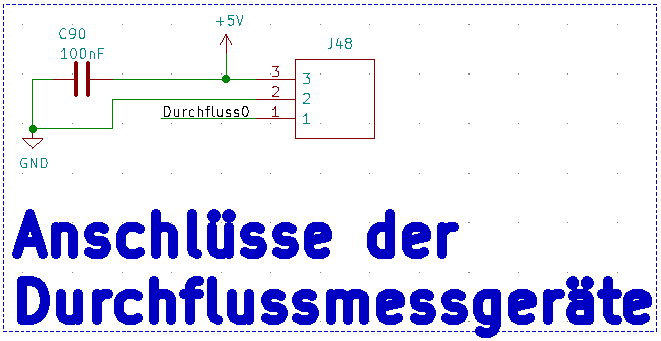
\includegraphics[width=0.6\textwidth]{graphics/Schema_Durchflussmessgeraete.png}
	\caption{Schema der Durchflussmessgeräte.}
	\label{fig:Schema_Durchflussmessgeräte}
\end{figure}

\paragraph{Funktionsbeschrieb der Schaltung}\mbox{}

Die Durchflussmessgeräte haben drei Anschlüsse. Zum einen ist dies einen Speisungseingang von 5V und eine Groundleitung. Der dritte Pin der Durchflussmessgeräte ist ein Signalpin, welcher bei Durchfluss ein gepulstes Signal mit 5V und 50\% Duty-Cycle ausgibt. Da dieses Signal direkt vom Mikrocontroller ausgewertet werden kann, ist keine weitere Elektronik erforderlich. Zur Auswertung der Signale werden gemäss Kapitel \ref{subsec:Mikrocontroller} wiederum Digitalpins als Eingänge verwendet. \cite{five__tools_store_us_nodate}  